\documentclass[a4paper, twocolumn, titlepage, 10pt]{article}
\usepackage{amsmath, graphicx, gensymb, float}
\usepackage{mathtools}
\usepackage{listings}
\usepackage{lettrine}
\usepackage{tabularx}
\usepackage{array}
\newcolumntype{O}{>{\centering\arraybackslash}m{0.8cm}}
\newcolumntype{L}{>{\centering\arraybackslash}m{1.8cm}}
\title{\textbf{ECSE 307 Linear Systems and Control} \linebreak Lab 4 Report}
\author{Hai XU, 260661832 \and Wenjie WEI, 260685967}
\date{October 25$^{th}$, 2017}
\usepackage{color} %red, green, blue, yellow, cyan, magenta, black, white
\usepackage{inconsolata}
\definecolor{mygreen}{RGB}{28,172,0} % color values Red, Green, Blue
\definecolor{mylilas}{RGB}{170,55,241}

\lstset{language=Matlab,%
	%basicstyle=\color{red},
	basicstyle=\ttfamily,
	breaklines=true,%
	morekeywords={matlab2tikz},
	keywordstyle=\color{blue},%
	morekeywords=[2]{1}, keywordstyle=[2]{\color{black}},
	identifierstyle=\color{black},%
	stringstyle=\color{mylilas},
	commentstyle=\color{mygreen},%
	showstringspaces=false,%without this there will be a symbol in the places where there is a space
	numbers=left,%
	numberstyle={\tiny \color{black}},% size of the numbers
	numbersep=9pt, % this defines how far the numbers are from the text
	emph=[1]{for,end,break},emphstyle=[1]\color{red}, %some words to emphasise
	%emph=[2]{word1,word2}, emphstyle=[2]{style},    
}

\begin{document}
	\maketitle
	\section{Introduction}
		\lettrine{T}{his} lab introduces the methodologies to analyze the behavior of a dynamic system. Proportional, Integral, and Derivative (PID) controls are so far the most common type of controllers that are used. They are simple yet still able to give promising performance. Figure \ref{PIDData} shows what will happen if a PID controller is implemented.
		\begin{figure}[H]
			\centering
			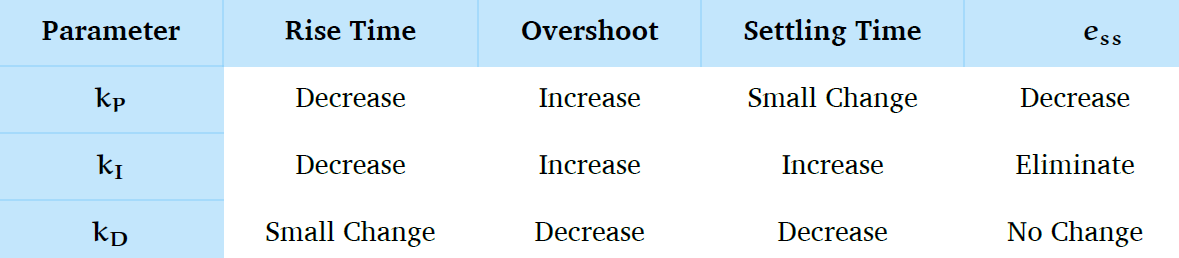
\includegraphics[width=\linewidth]{PIDData}
			\caption{Key Changes that PID Systems Can Bring}
			\label{PIDData}
		\end{figure}
	\section{Finding the PID Gains}
		Consider a system transfer function as below:
		$$
			G(s) = \frac{1}{(s+1)(s+2)(s+3)}
		$$
		Plot the step response using MATLAB. The step response of the system is shown in Figure \ref{G_step}:
		\begin{figure}[H]
			\centering
			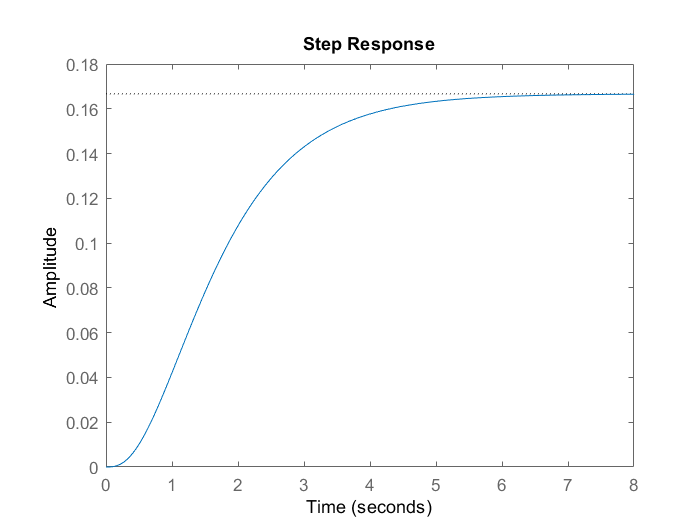
\includegraphics[width=\linewidth]{G_step}
			\caption{Step Response of System G(s)}
			\label{G_step}
		\end{figure}
		
		Apply the MATLAB command:
		\begin{lstlisting}[frame = single, numbers=none]
stepinfo(G);
		\end{lstlisting}
		A vector containing some critical values will be generated. To find the steady state error $e_{ss}$, apply Final Value Theorem which is stated as below:
		\begin{equation}
			\lim\limits_{t \to \infty} y(t) = \lim\limits_{s \to \infty} sX(s)H(s)
			\label{fvt}
		\end{equation}
		Therefore, it can be calculated that $\lim\limits_{t \to \infty} y(t) = \frac{1}{6}$ which leads to the fact that $e_{ss} = \frac{5}{6} = 83.333\%$
		Table \ref{trtsmptable} shows the most critical data for future analysis of the system:
		\begin{table}[H]
			\centering
			\begin{tabular}{c c c c}
				$e_{ss}$ & $t_r$ & $t_s$ & $M_p$ \\
				83.33\% & 2.7428 & 5.0039 & 0
			\end{tabular}
			\caption{Table of Some Critical Values}
			\label{trtsmptable}
		\end{table}
		
		Next, the root locus plot will be needed to explore the stability of the system if we change the gain of the system.
		\begin{figure}[H]
			\centering
			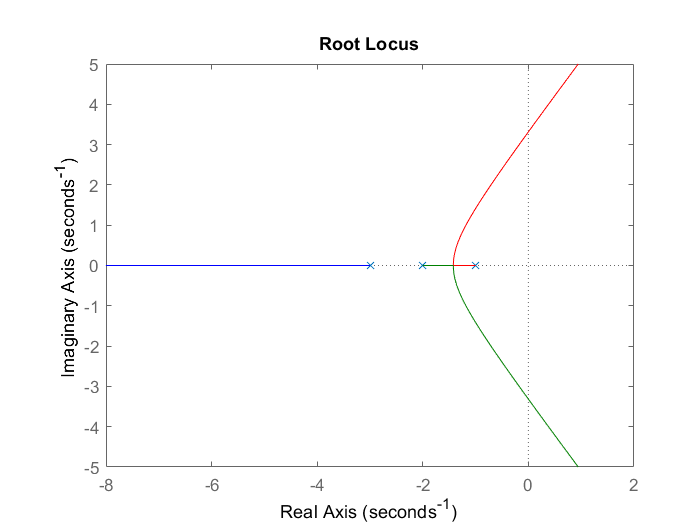
\includegraphics[width=\linewidth]{rlocus}
			\caption{Root-Locus Plot of the System}
			\label{rlocusG}
		\end{figure}
		
		Figure \ref{rlocusG} shows the root locus plot of the system G(s). From the MATLAB plot, we can find that at the marginal stability, gain $K = 60$ and frequency $\omega = 3.31 rad/s$.
		
		Using the information above, we are able to design a stable system with a proper gain. However, as can be seen from Table \ref{trtsmptable}, the rising time $t_r$ is really large, which means that this system responds slowsly to input signals. Idealy, we would like to design a controller that reduces the rise time, settling time, and eliminates the steady-state error. According to Figure \ref{PIDData}, a proportional controller decreases the rising time, and reduces the steady state error as well. Add a proportional controller by implementing the MATLAB code in the Section 6.2 of the Appendix, and find the step response characteristics for $k_p = 40$.
		\begin{figure}[H]
			\centering
			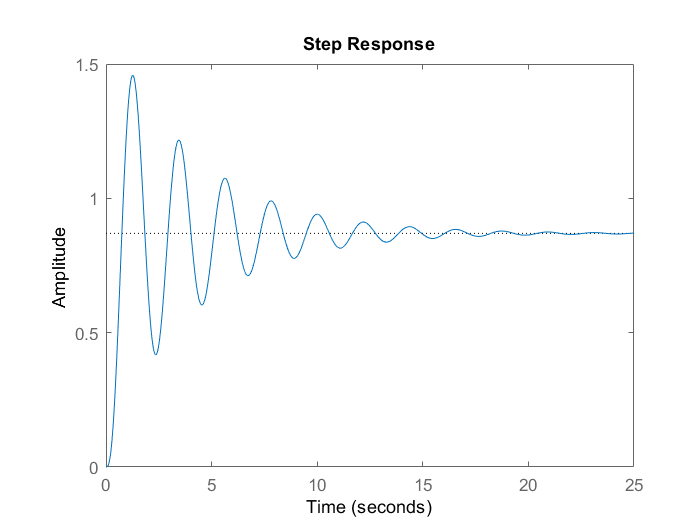
\includegraphics[width=\linewidth]{StepPC}
			\caption{Step Response of the P-Controller}
			\label{steppc}
		\end{figure}
		
		Figure \ref{steppc} shows the step response and Table shows the key response characteristics of the system after adding a proportional controller. 
		\begin{table}[H]
			\centering
			\begin{tabular}{c c c c}
				$e_{ss}$ & $t_r$ & $t_s$ & $M_p$ \\
				13.043\% & 0.4368 & 15.6105 & 67.6273
			\end{tabular}
			\caption{Table of the Key Characteristics of the P-Controller}
			\label{responseCharPC}
		\end{table}
		
		\begin{figure}[H]
			\centering
			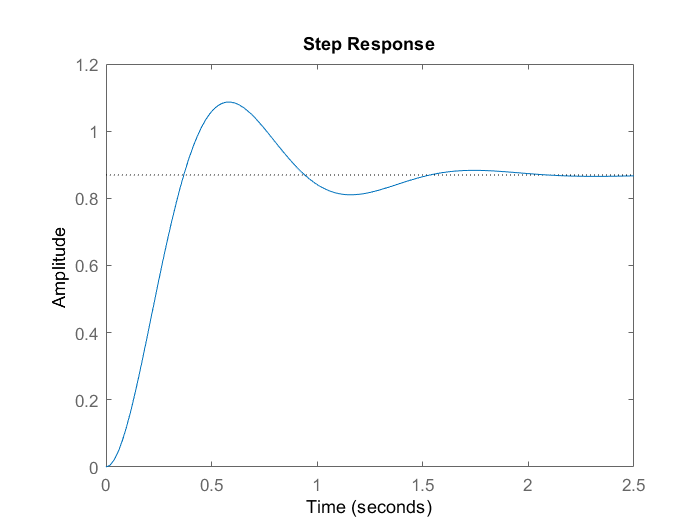
\includegraphics[width=\linewidth]{StepPD}
			\caption{Step Response of the PD Controller}
			\label{StepPD}
		\end{figure}
		Compare the data in Table \ref{responseCharPC} and \ref{trtsmptable}, it can be seen clearly that by adding the P-Controller, the rise time of the system $t_r$ gets much smaller. However, the giant overshoot of this system makes the system not as stable as it was before, and the settling time becomes much longer meaning that it is taking longer for the system to reach a steady state.
		
		Add another derivative controller using the code in Appendix 6.3, we can add the derivative controller and implement a PD controller. Plot the step response of the system as is shown in Figure \ref{StepPD}.
		
		Use MATLAB, list the key characteristics of this PD-Controller as is shown in Table \ref{responseCharPD} as follows:
		%====================
		%TODO: STEADY STATE ERROR
		%====================
		\begin{table}[H]
			\centering
			\begin{tabular}{c c c c}
				$e_{ss}$ & $t_r$ & $t_s$ & $M_p$ \\
				13.043\% & 0.2494 & 1.4318 & 24.9544
			\end{tabular}
			\caption{Table of the Key Characteristics of the PD-Controller}
			\label{responseCharPD}
		\end{table}
	
		As is clearly shown from the tables, the PD controller has a much better performance. Compared with the data from Table \ref{trtsmptable}, the rising time $t_r$ settling time $t_s$ decreased significantly, and maximum overshoot $M_p$ increased obviously. Now the system responds to the input faster, at the cost of being a little bit less stable due to the overshoot. In addition, the output of the system reaches stable state more quickly.
		
		Using the code in 6.4 in Appendix, we can keep the proportional controller and add the integral controller. Plot the step response of the PI controller using MATLAB shown in Figure \ref{StepPI}.
		\begin{figure}[H]
			\centering
			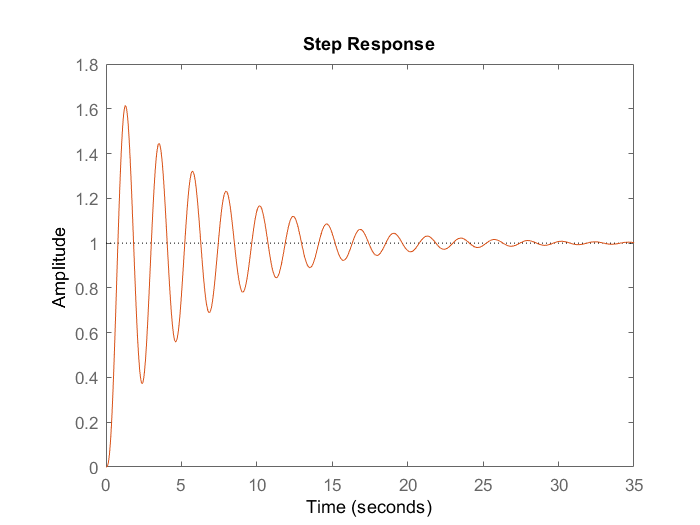
\includegraphics[width=\linewidth]{StepPI}
			\caption{Step Response of the PI Controller}
			\label{StepPI}
		\end{figure}
	
		Use MATLAB, list the key characteristics of this PI-Conntroller as is shown in Table 4 as follows:
		\begin{table}[H]
			\centering
			\begin{tabular}{c c c c}
				$e_{ss}$ & $t_r$ & $t_s$ & $M_p$ \\
				0 & 0.4593 & 23.6832 & 61.3913
			\end{tabular}
			\caption{Table of the Key Characteristics of the PI-Controller}
			\label{responseCharPI}
		\end{table}
	
		Compare the data from Table \ref{responseCharPI} with that from Table \ref{trtsmptable}. It can be seen that the rising time $t_r$ decreased significantly. However, the maximum overshoot $M_p$ and the settling time $t_s$ increased significantly. Meaning that although the system responds faster to input, it takes a long time to reach steady state, as well as increases instablities. 
		
		Change the value of $k_p$, and observe the step response of the PI Controller as is shown in Figure \ref{StepPI_diffKp}. 
		\begin{figure}[H]
			\centering
			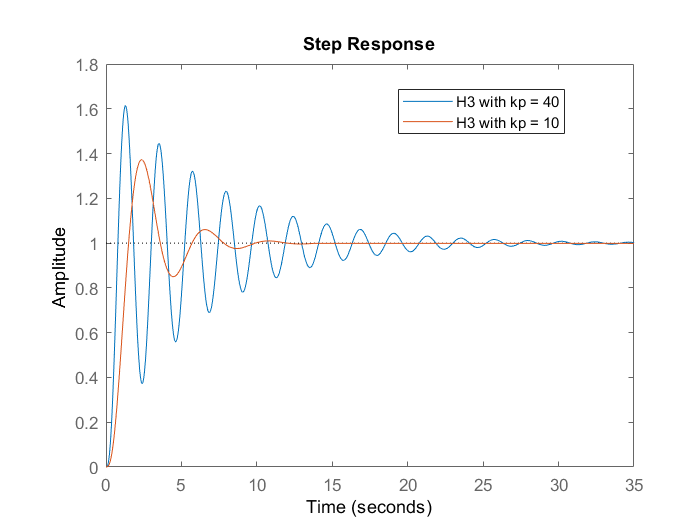
\includegraphics[width=\linewidth]{StepPI_diffKp}
			\caption{Step Response of the PI Controller with Different $k_p$ Values}
			\label{StepPI_diffKp}
		\end{figure}
	
		The yellow plot on the graph shows the step response of the PI controller with $k_p = 10$. It is clearly shown that the rising time of the system increases while the maximum overshoot and the settling time decrease. Whether or not we should keep $k_p=40$, we need to determine how fast, or how stable we want the system to respond to an input signal and set the value accordingly.
		
		Implement a PID controller by using the MATLAB code in Appendix 6.5. The step response plot is shown in Figure \ref{StepPID}.
		\begin{figure}[H]
			\centering
			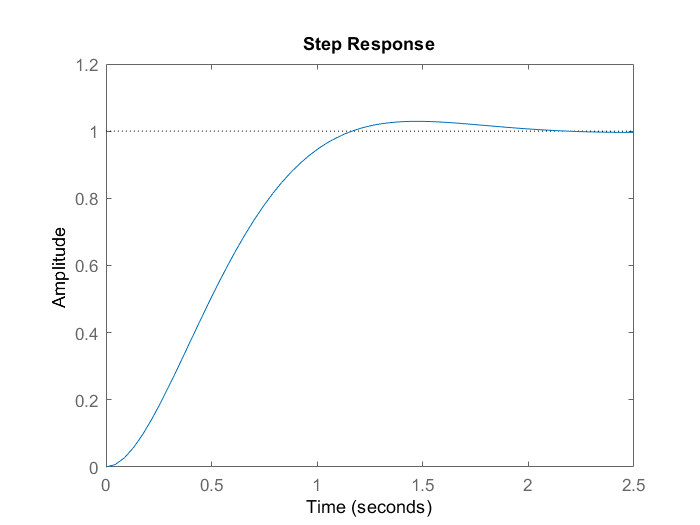
\includegraphics[width=\linewidth]{StepPID}
			\caption{Step Response of the PID Controller}
			\label{StepPID}
		\end{figure}
	
		Table \ref{responseCharPID} shows the critical characteristics of the system. 
		\begin{table}[H]
			\centering
			\begin{tabular}{c c c c}
				$e_{ss}$ & $t_r$ & $t_s$ & $M_p$ \\
				0 & 0.7352 & 1.7392 & 2.9293
			\end{tabular}
			\caption{Table of the Key Characteristics of the PID-Controller}
			\label{responseCharPID}
		\end{table}
	
		Compare with the data we obtained from different controllers we obtained before. It can be clearly shown that by using a PID controller, the rising time $t_r$ is very small. Although it is larger than that of other controllers, it is still promising since it is much smaller than the rising time of the open loop system $G(s)$. Also, By using the PID Controller, the system becomes smaller since the overshoot and settling time is decreased significantly.
		
		A complete table of the step response characteristics of the PID Controllers can be found in Appendix Section 6.6. From the table, we can verify the effect of different controllers shown in Figure \ref{PIDData} is true.
	\section{Automatic PID Tuning with MATLAB}
		In this section we start to consider G(s) defined in Section 1. For the unit feedback controlled system, we use the code in Appendix 6.5 to plot the step response for each controller.
		
		By combining the type P and disturbance rejection, we get the step response shown in Figure \ref{p-rej-step}.
		\begin{figure}[H]
			\centering
			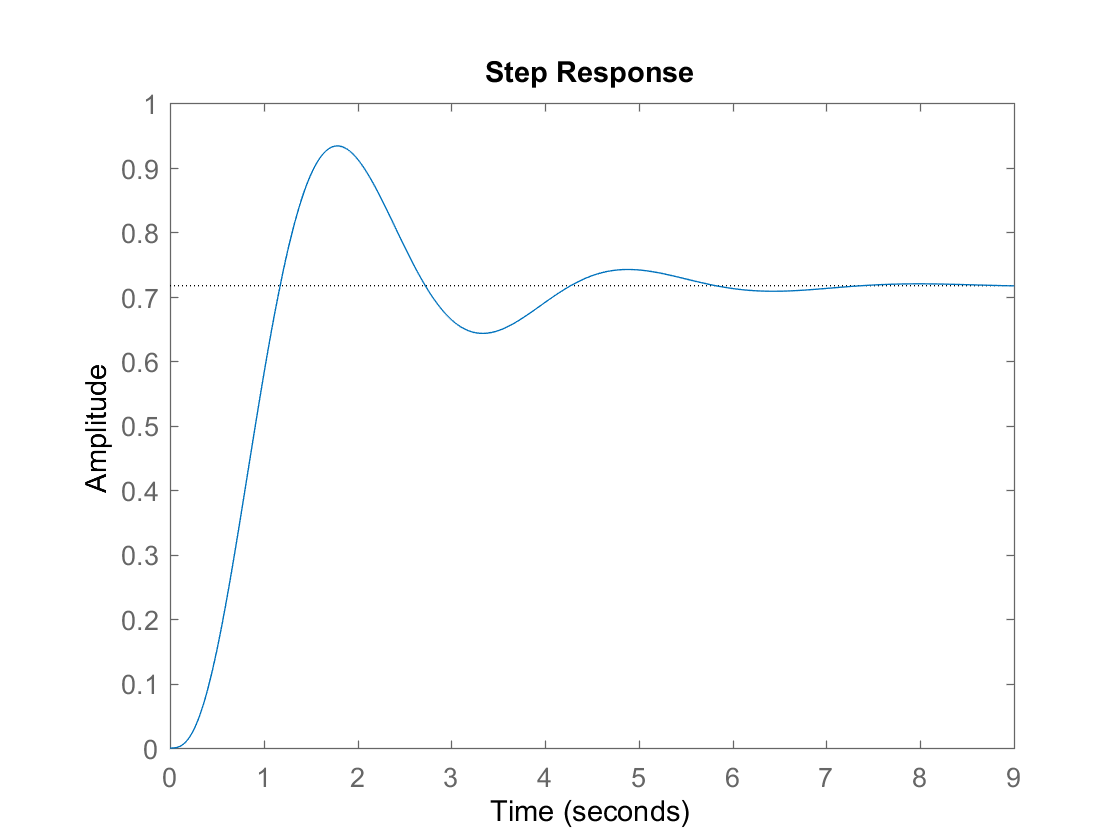
\includegraphics[width=\linewidth]{p-rej-step}
			\caption{Step response of the type P-Disturbance Rejection}
			\label{p-rej-step} 
		\end{figure}
		
		By combining the type P and Reference Tracking, we get the step response shown in Figure \ref{p-track-step}.
		\begin{figure}[H]
			\centering
			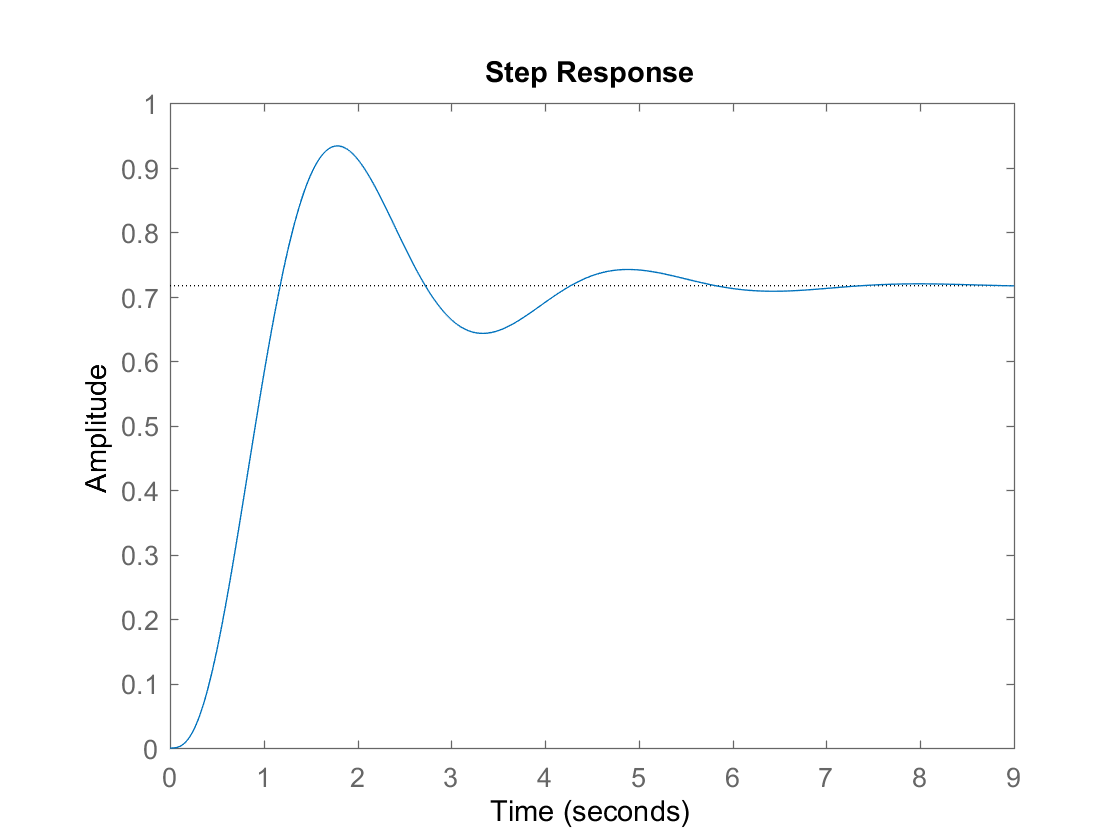
\includegraphics[width=\linewidth]{p-track-step}
			\caption{Step response of the type P-Reference Tracking}
			\label{p-track-step} 
		\end{figure}
		By combining the type P and Balanced, we get the step response shown in Figure \ref{p-balance-step}. 
		\begin{figure}[H]
			\centering
			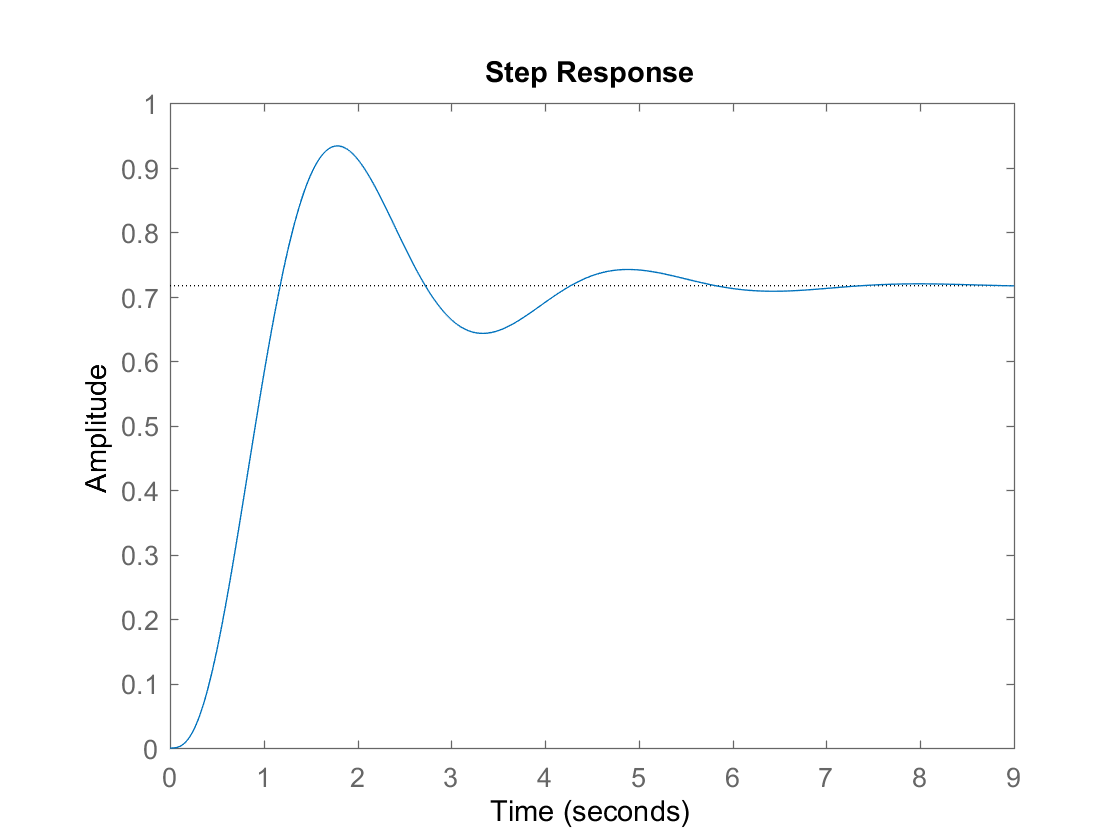
\includegraphics[width=\linewidth]{p-balance-step}
			\caption{Step response of the type P-Balanced Tracking}
			\label{p-balance-step} 
		\end{figure}
		By combining the type I and Disturbance Rejection, we get the step response shown in Figure \ref{I-rej-step}.
		\begin{figure}[H]
			\centering
			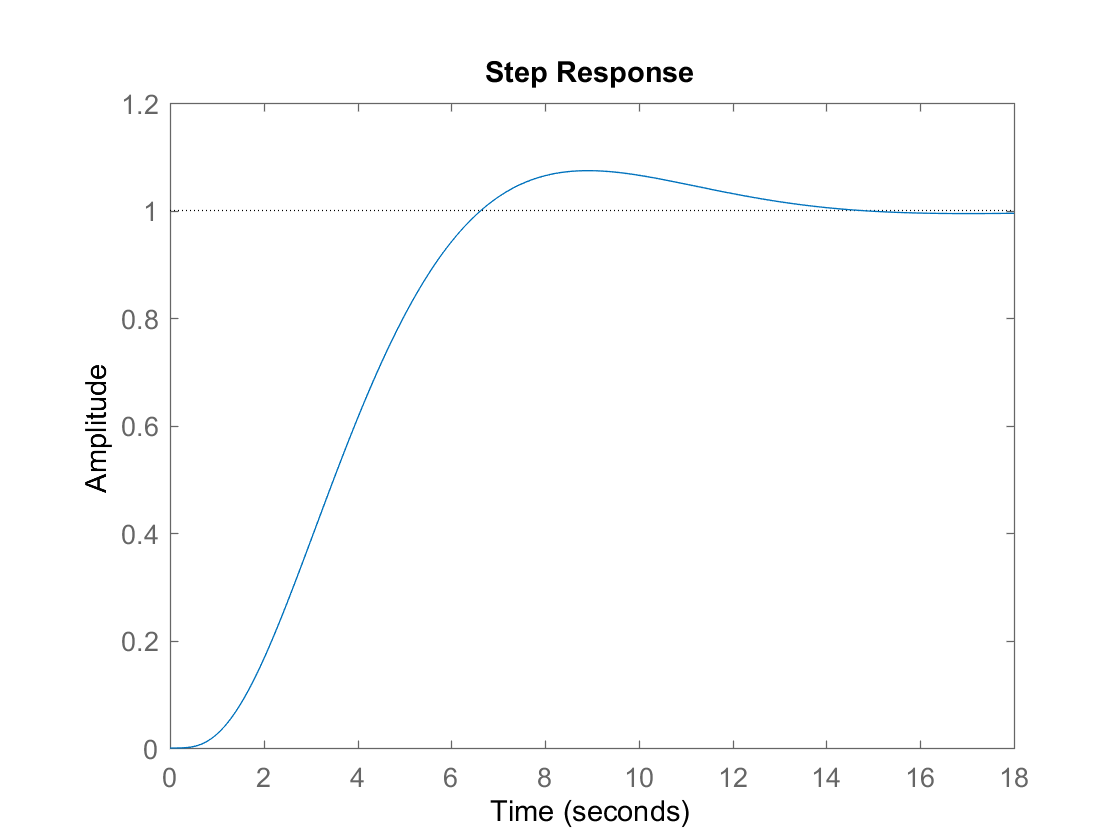
\includegraphics[width=\linewidth]{I-rej-step}
			\caption{Step response of the type I-Disturbance Rejection}
			\label{I-rej-step} 
		\end{figure}
		By combining the type I and Reference Tracking, we get the step response shown in Figure \ref{I-track-step}.
		\begin{figure}[H]
			\centering
			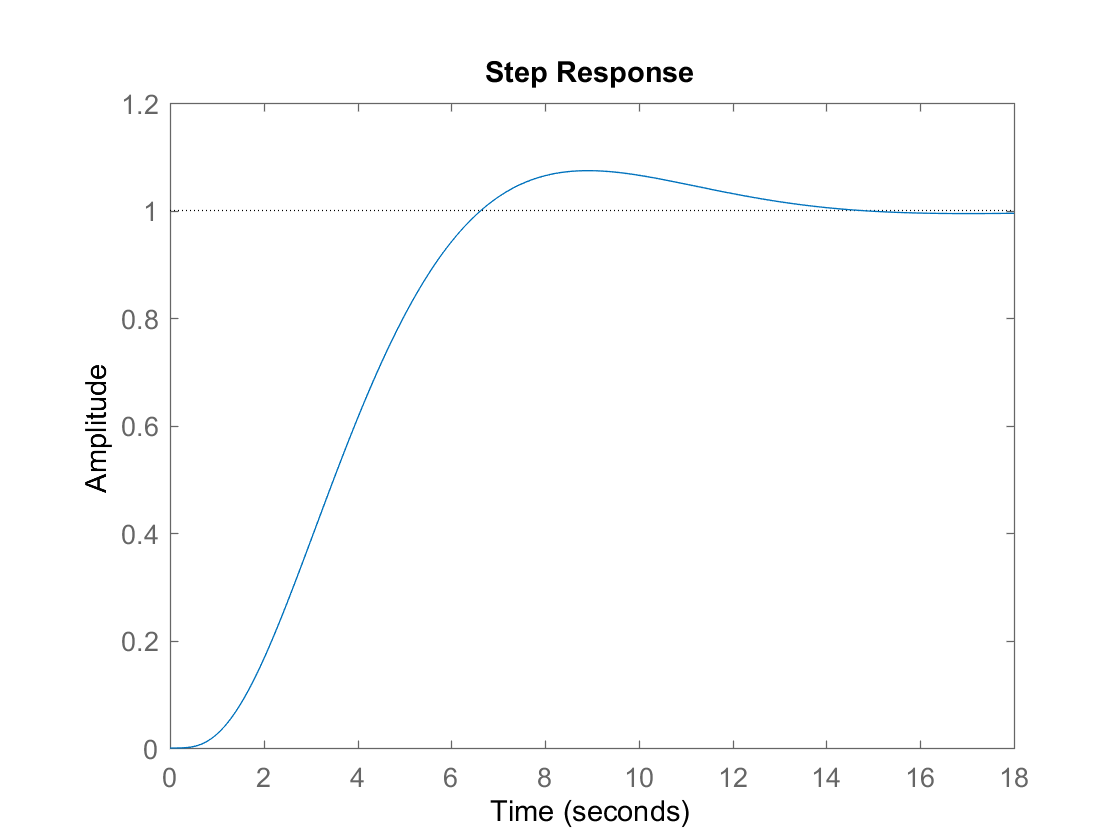
\includegraphics[width=\linewidth]{I-track-step}
			\caption{Step response of the type I-Reference Tracking}
			\label{I-track-step} 
		\end{figure}
		By combining the type I and Balanced, we get the step response shown in Figure \ref{I-balance-step}.
		\begin{figure}[H]
			\centering
			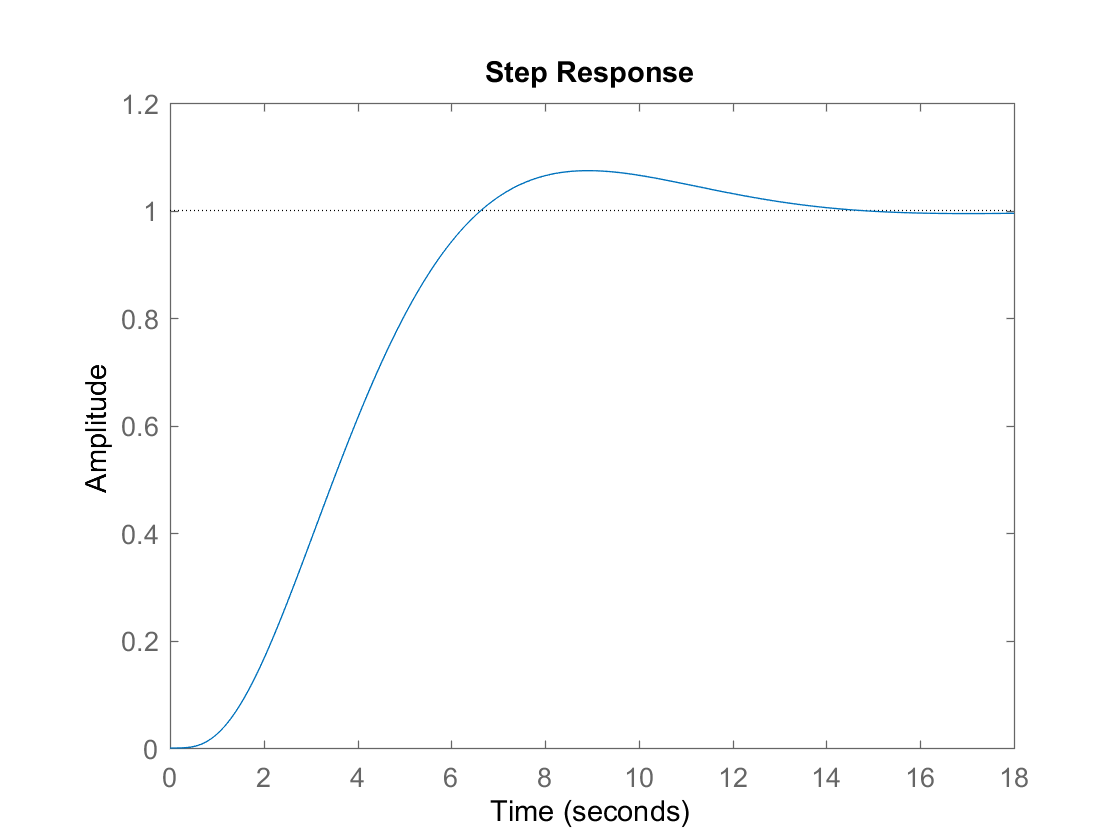
\includegraphics[width=\linewidth]{I-balance-step}
			\caption{Step response of the type I-Balanced}
			\label{I-balance-step}
		\end{figure}
		By combining the type PI and Disturbance Rejection, we get the step response shown in Figure \ref{PI-rej-step}.
		\begin{figure}[H]
			\centering
			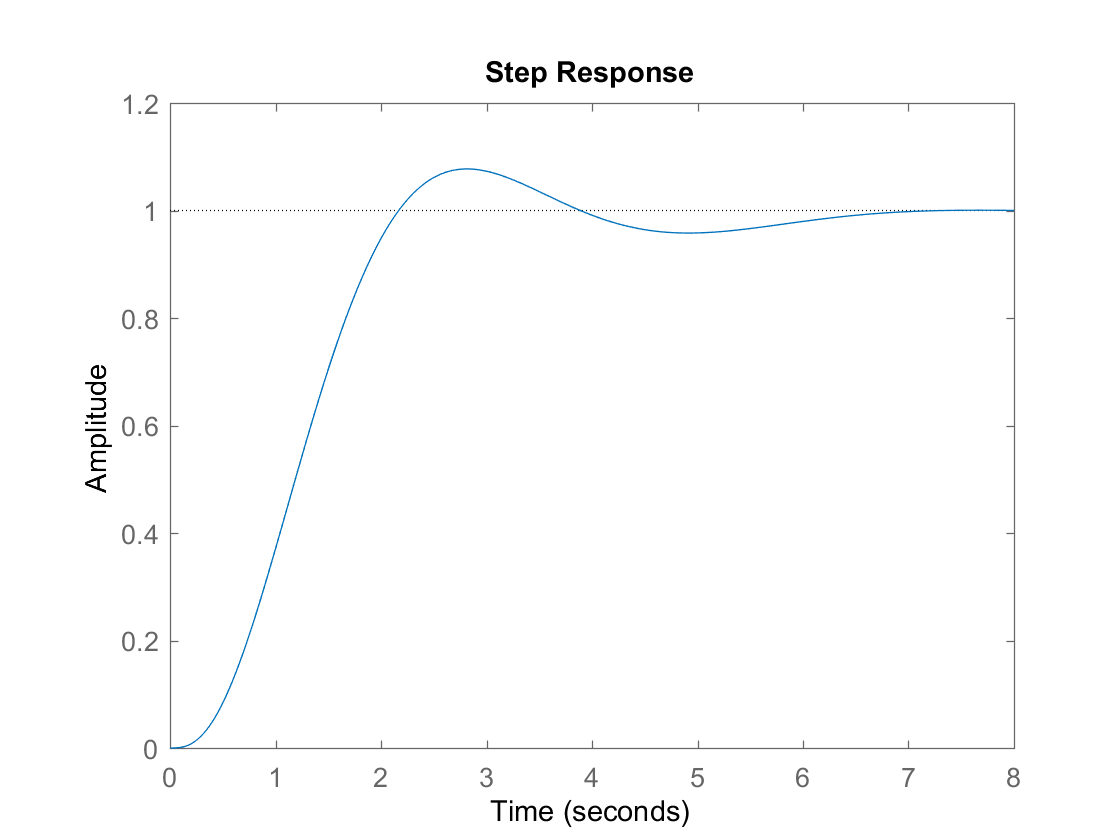
\includegraphics[width=\linewidth]{PI-rej-step}
			\caption{Step response of the type PI-Disturbance Rejection}
			\label{PI-rej-step}
		\end{figure}
		By combining the type PI and Reference Tracking, we get the step response shown in Figure \ref{PI-track-step}.
		\begin{figure}[H]
			\centering
			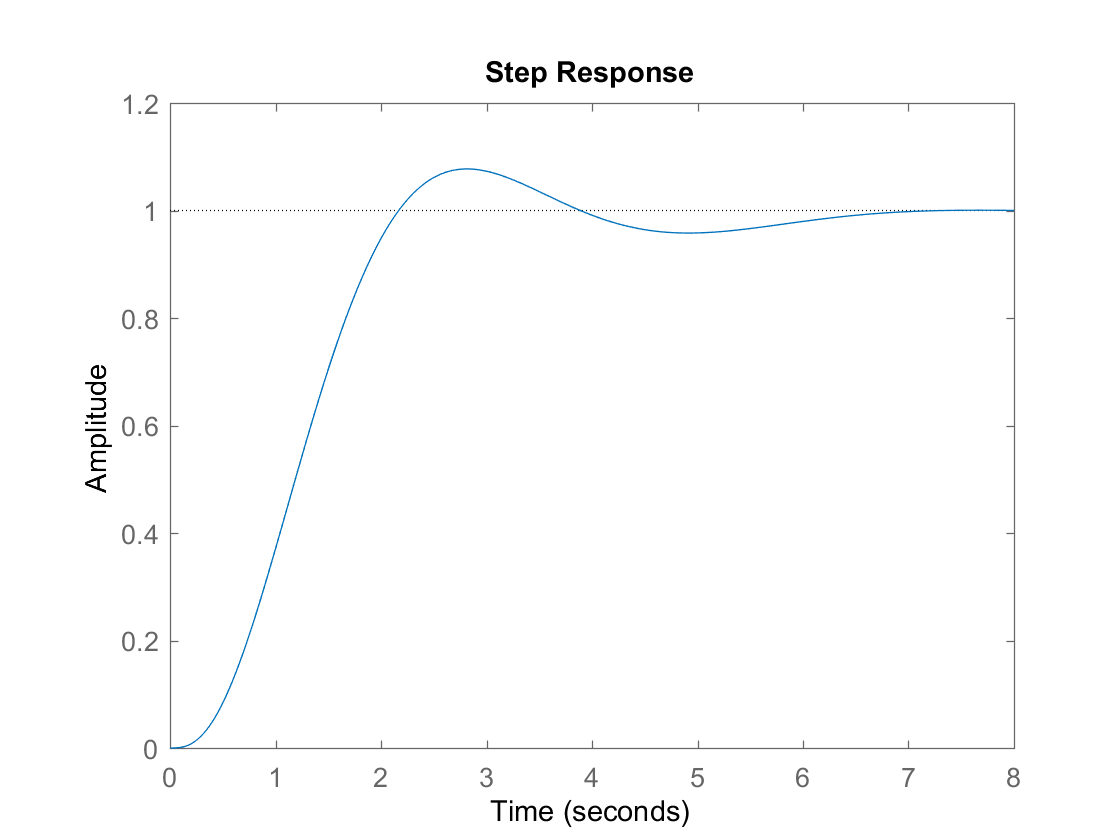
\includegraphics[width=\linewidth]{PI-track-step}
			\caption{Step response of the type PI-Reference Tracking}
			\label{PI-track-step}
		\end{figure}
		By combining the type PI and Balanced, we get the step response shown in Figure \ref{PI-balance-step}.
		\begin{figure}[H]
			\centering
			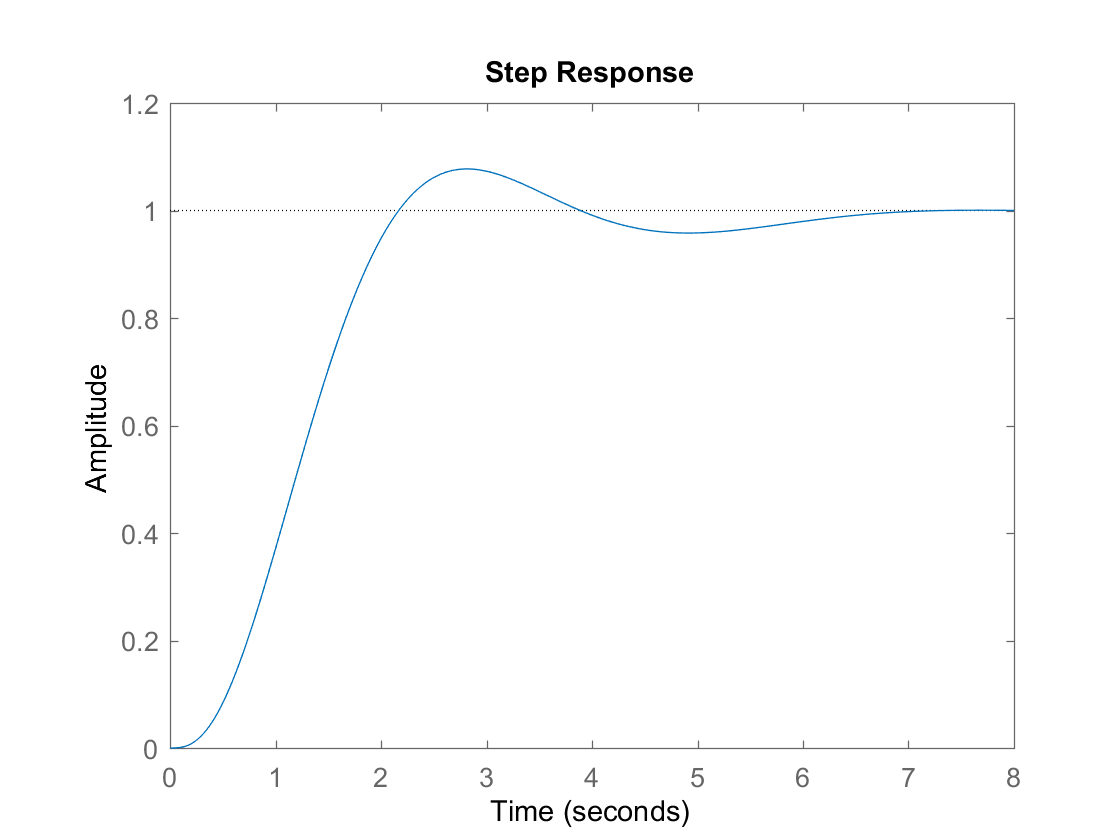
\includegraphics[width=\linewidth]{PI-balance-step}
			\caption{Step response of the type PI-Balanced}
			\label{PI-balance-step}	
		\end{figure}
		By combining the type PD and Disturbance Rejection, we get the step response shown in Figure \ref{PD-rej-step}.
		\begin{figure}[H]
			\centering
			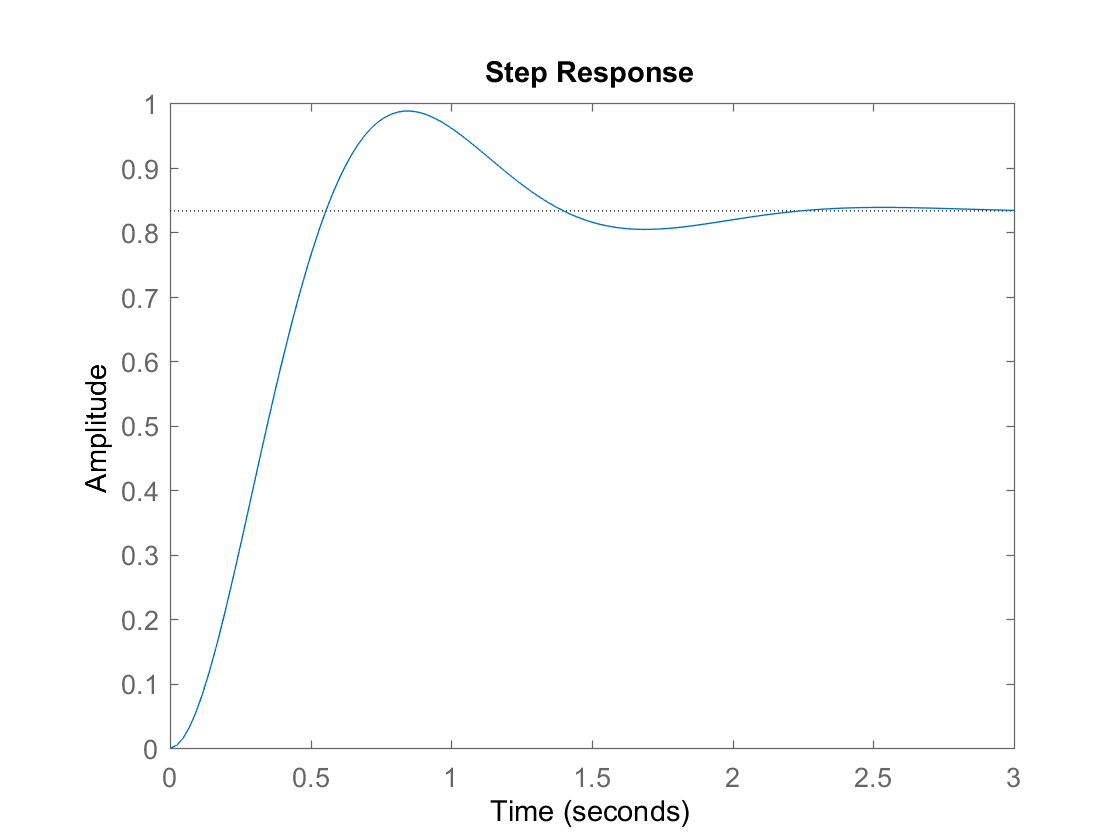
\includegraphics[width=\linewidth]{PD-rej-step}
			\caption{Step response of the type PD-Disturbance Rejection}
			\label{PD-rej-step}
		\end{figure}	
		By combining the type PD and Reference Tracking, we get the step response shown in Figure \ref{PD-track-step}.
		\begin{figure}[H]
			\centering
			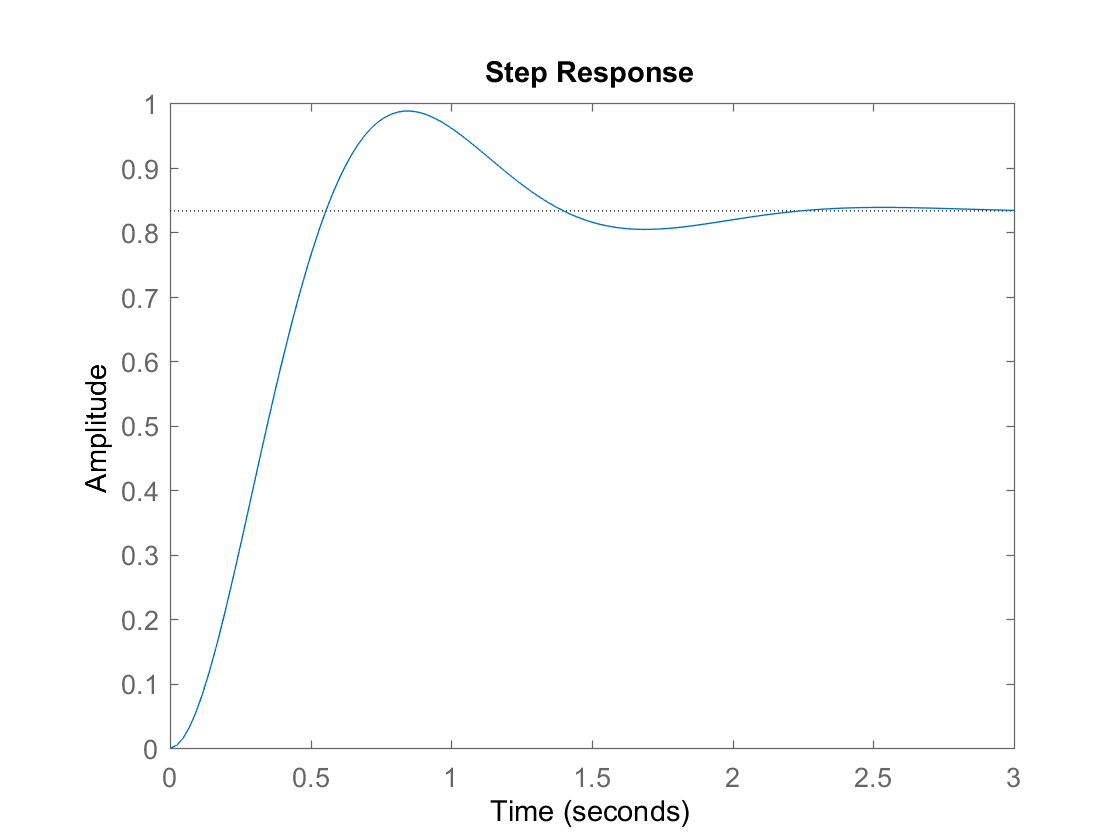
\includegraphics[width=\linewidth]{PD-track-step}
			\caption{Step response of the type PD-Reference Tracking}
			\label{PD-track-step}
		\end{figure}
		By combining the type PD and Balanced, we get the step response shown in Figure \ref{PD-balance-step}.
		\begin{figure}[H]
			\centering
			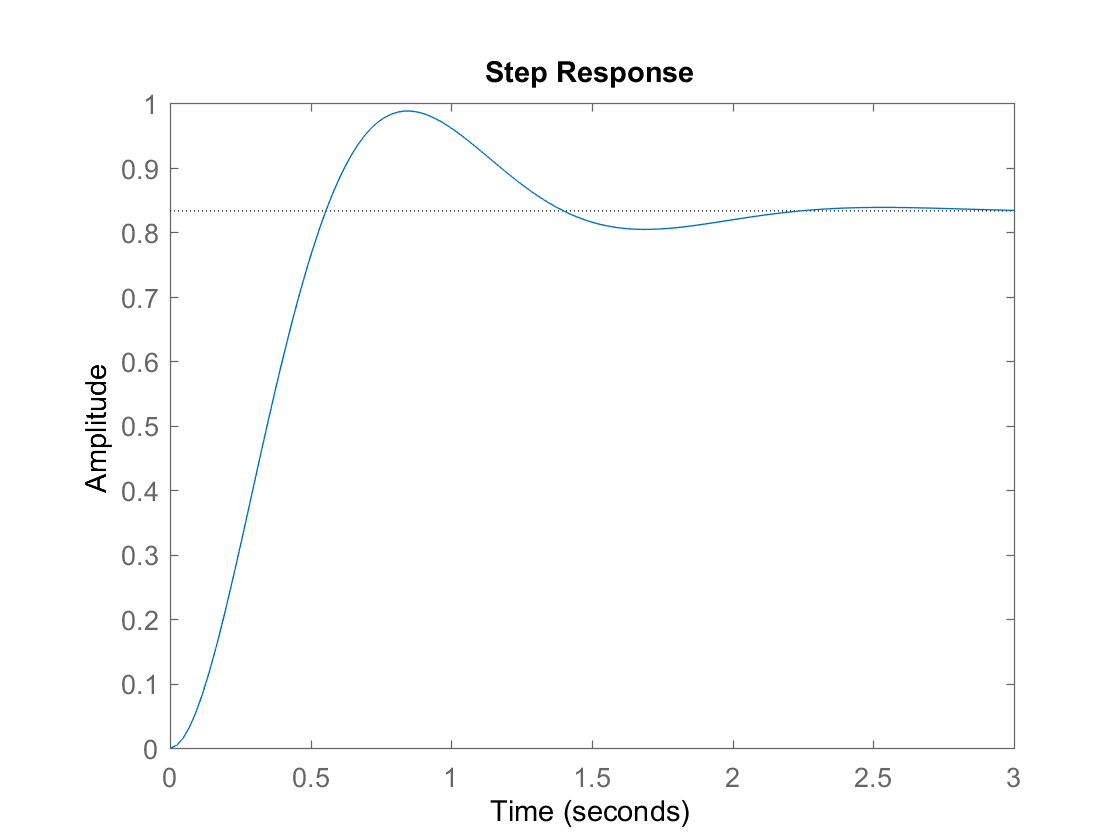
\includegraphics[width=\linewidth]{PD-balance-step}
			\caption{Step response of the type PD-Balanced}
			\label{PD-balance-step}
		\end{figure}
		By combining the type PID and Disturbance Rejection, we get the step response shown in Figure \ref{PID-rej-step}.
		\begin{figure}[H]
			\centering
			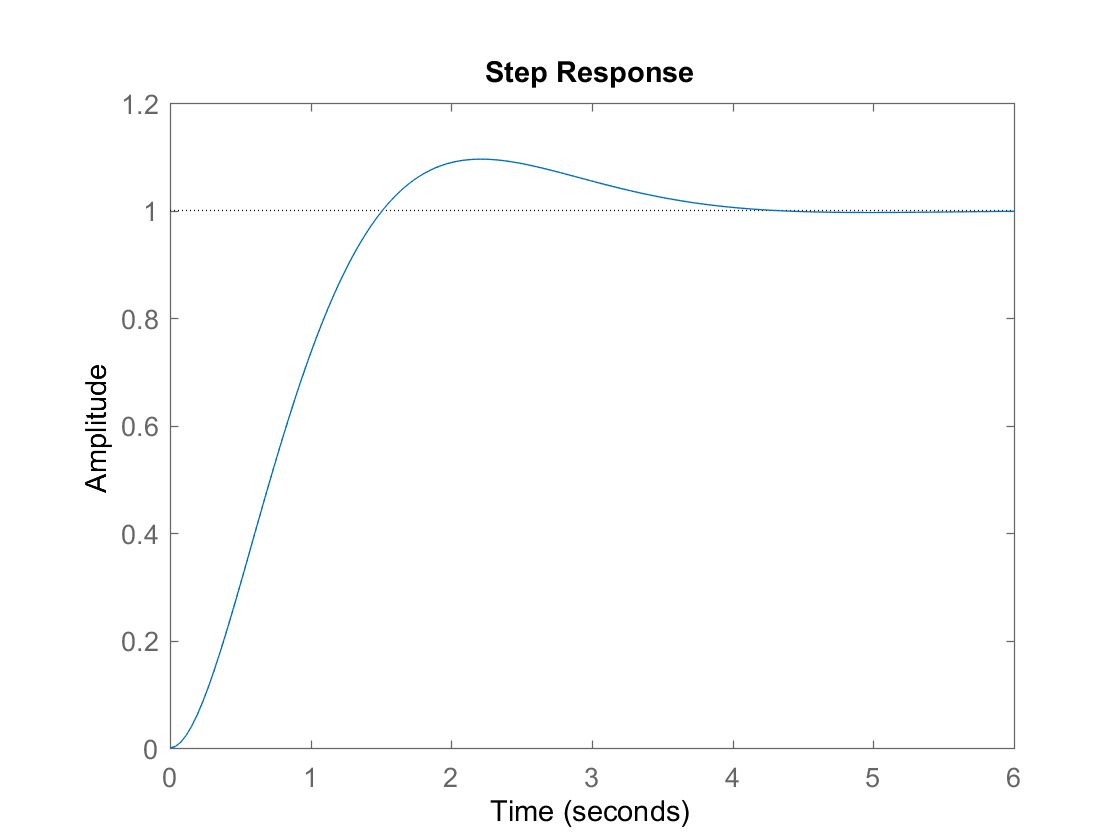
\includegraphics[width=\linewidth]{PID-rej-step}
			\caption{Step response of the type PID-Disturbance Rejection}
			\label{PID-rej-step}
		\end{figure}
		By combining the type PID and Reference Tracking, we get the step response shown in Figure \ref{PID-track-step}.
		\begin{figure}[H]
			\centering
			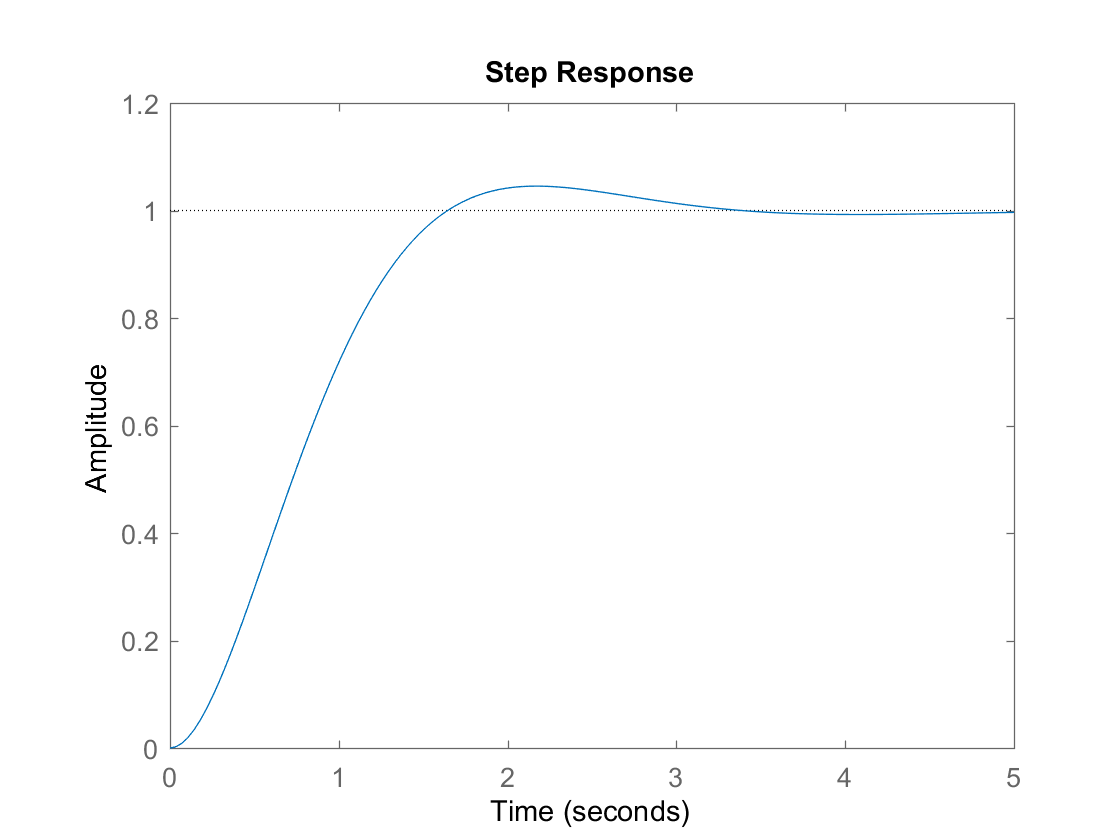
\includegraphics[width=\linewidth]{PID-track-step}
			\caption{Step response of the type PID-Reference Tracking}
			\label{PID-track-step}
		\end{figure}
		By combining the type PID and Balanced, we get the step response shown in Figure \ref{PID-balance-step}.
		\begin{figure}[H]
			\centering
			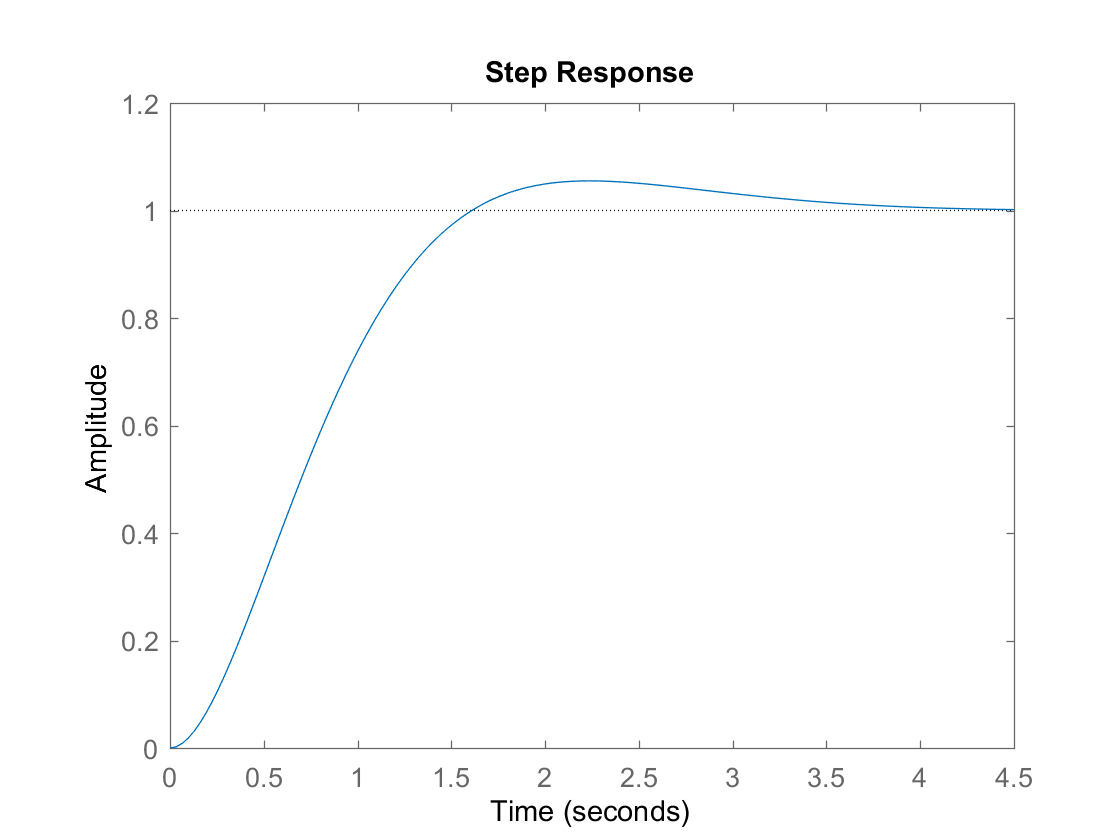
\includegraphics[width=\linewidth]{PID-balance-step}
			\caption{Step response of the type PID-Balanced}
			\label{PID-balance-step}
		\end{figure}	
		The values of $K_P$, $K_I$ and $K_D$ for each combination of the options are shown in the table below.
		\begin{table}[H]
			\centering
			\begin{tabular}{O | L| L | L}
				Type & Disturbance Rejection & Reference Tracking & Balanced \\
				\hline
				P	& $k_p = 15.2$ & $k_p = 15.2$ & $k_p = 15.2$ \\ 
				\hline
				I  & $k_I = 1.843$ & $k_I = 1.843$ & $k_I = 1.843$\\
				\hline
				PI & $k_p = 7.586$ $k_I = 5.029$ &$k_p = 7.586$ $k_I = 5.029$&$k_p = 7.586$ $k_I = 5.029$	\\
				\hline
				PD&	$k_p = 29.88$ $k_D = 14.85$&$k_p = 29.88$ $k_D = 14.85$&$k_p = 29.88$ $k_D = 14.85$\\
				\hline
				PID&$k_p = 12.54$ $k_I = 9.91$ $k_D = 3.97$&$k_p = 12.54$ $k_I = 9.91$ $k_D = 3.97$&	$k_p = 12.54$ $k_I = 9.91$ $k_D = 3.97$
			\end{tabular}
			\caption{Table of $K_P$, $K_I$ and $K_D$ for each combination of the options}
			\label{combinations}
		\end{table}
	\section{PID Tuning with Ziegler Nichols Method - The Ultimate Sensitivity Approach}
	
	A proportional controller is used to use the ultimate sensitivity approach. Based on the evaluation of the amplitude and frequency of the system at the limit of stability, the proportional gain $K_p$ is increased until the system becomes marginally stable. This gain is defined as the ultimate gain $K_u$ and the corresponding period is defined similarly as the ultimate period $P_u$. The tuning parameters are determined according to Table \ref{ZNTuning}.
	\begin{table}[H]
		\centering
		\begin{tabular}{c c}
			Type & Optimum Gain \\
			P & $k_p = 0.5K_u$ \\
			PI & $k_p = 0.45K_u, k_I = \frac{1.2}{P_u}$ \\
			PID & $k_p=1.6K_u, k_I = \frac{1}{0.5P_u}, k_D = 0.125P_u$
		\end{tabular}
		\caption{Ziegler-Nichols Tuning for PID Controller Based on the Ultimate Sensitivity Mode}
		\label{ZNTuning}
	\end{table}

	Now consider the transfer function $G(s)$ determined in Section 2. We would like to find the P, PI, and PID controller gains using the ultimate sensitivity method. First of all, use MATLAB, plot the Bode Plot and the Root Locus of this open-loop system to find $k_u$ and $P_u$. 
	\begin{figure}[H]
		\centering
		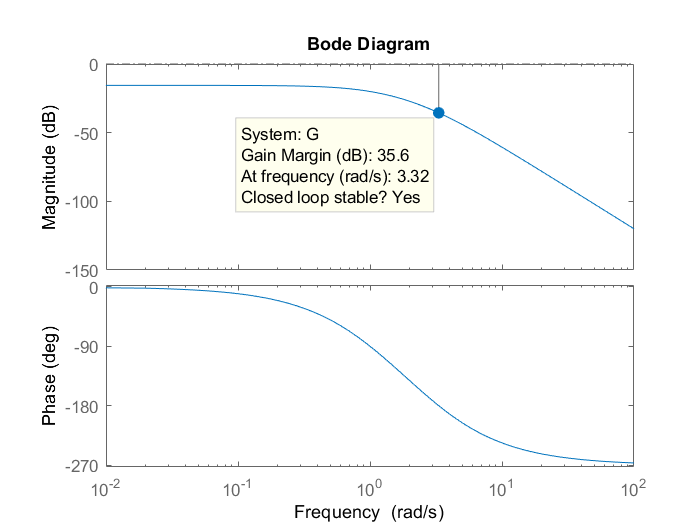
\includegraphics[width=\linewidth]{bode}
		\caption{Bode Plot of Open-Loop System $G(s)$}
		\label{bode}
	\end{figure}
	The Bode Plot of $G(s)$ is shown in Figure \ref{bode}. The value of the gain margin and frequency are shown in the figure. The gain margin $G_m = 35.6dB$ and $\omega _m = 3.32rad/s$. Now we can compute the ultimate gain:
	\begin{align*}
		G_m &= 20log_{10}K_u \\
		K_u &=  10^{\frac{G_m}{20}} = 60.256
	\end{align*}
	and the ultimate period:
	$$
		P_u = \frac{2\pi}{\omega_m} = 1.893
	$$
	
	Refer to the marginal gain and frequency found in Section 2 from the Root-Locus Plot, it is easy to say that these data are the same. 
	
	Now we would like to design P, PI, and PID controller for $G(s)$ using the above data and Table \ref{ZNTuning}. For the P controller, $k_p = 0.5K_u = 30.128$. Define the controller as $k_p$, and implement in MATLAB using the following code and find the step response of the system shown in Figure \ref{step_p_zn}.
	\begin{lstlisting}[frame=single, numbers=none]
G = tf([1], [1 6 11 6]);
C_PID = pid(30.128, 0, 0);
open_loop_sys = series(C_PID, G);
H_sys = feedback(open_loop_sys, 1);
step(H_sys);
	\end{lstlisting}
	\begin{figure}[H]
		\centering
		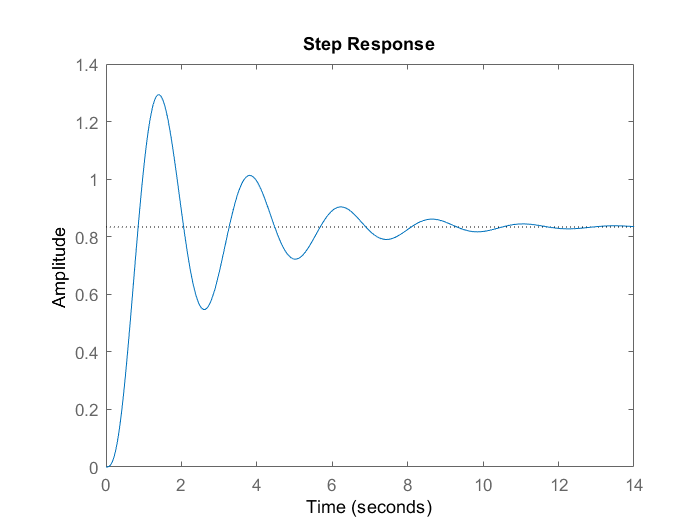
\includegraphics[width=\linewidth]{Step_P_ZNTuning}
		\caption{Step Response Calculated using Ziegler Nichols Tuning}
		\label{step_p_zn}
	\end{figure}
	
	Find the step response characteristics using MATLAB function stepinfo() again, and Table is obtained:
	\begin{table}[H]
		\centering
		\begin{tabular}{c c c c}
			$e_{ss}$ & $t_r$ & $t_s$ & $M_p$ \\
			16.608\% & 0.5031 & 9.9148 & 55.1082
		\end{tabular}
		\caption{Table of Step Response Characteristics of the P-Controller}
		\label{steptable_p_zn}
	\end{table}

	Similarly, we can implement a PI controller. Compute $k_p$ and $k_I$ again as follows:
	$$
		k_p = 0.45\times K_u = 27.115
	$$
	and
	$$
		k_I = \frac{1.2}{P_u} = 0.634
	$$
	
	Implement a PI controller in MATLAB using the code and the step response of the system is shown in Figure \ref{step_pi_zn}.
	\begin{lstlisting}[frame=single, numbers=none]
G = tf([1], [1 6 11 6]);
C_PID = pid(27.115, 0.634, 0);
open_loop_sys = series(C_PID, G);
H_sys = feedback(open_loop_sys, 1);
step(H_sys);
	\end{lstlisting}
	\begin{figure}[H]
		\centering
		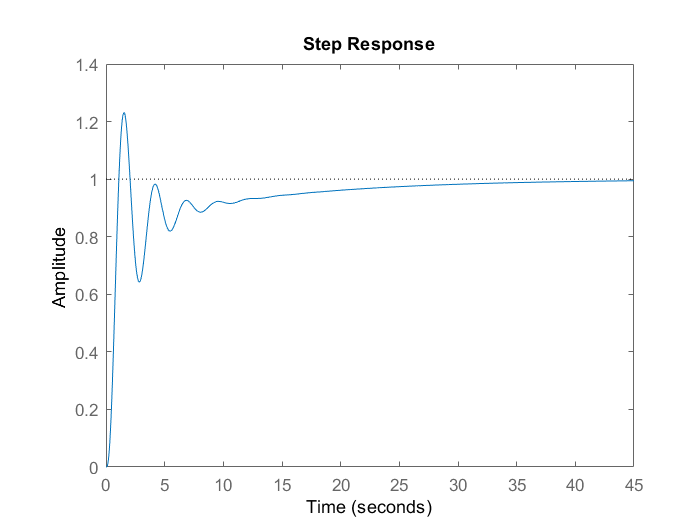
\includegraphics[width=\linewidth]{Step_PI_ZN}
		\caption{Step Response of PI Controller Plotted by MATLAB Using Ziegler Nichols Tuning}
		\label{step_pi_zn}
	\end{figure}
	
	Use the stepinfo() function to obtain the step response characteristic of this system.
	\begin{table}[H]
		\centering
		\begin{tabular}{c c c c}
			$e_{ss}$ & $t_r$ & $t_s$ & $M_p$ \\
			0 & 0.0513 & 78.301 & 62.814
		\end{tabular}
		\caption{Step Response Characteristic of the PI Controller Using Ziegler Nichols Tuning}
		\label{steptable_pi_zn}
	\end{table}
	Table \ref{steptable_pi_zn} shows the characteristics of the PI Controller which is obtained using the Ziegler Nichols Tuning approach. 
	
	A PID controller is obtained using the similar approach. First calculate the different parameters $k_p$, $k_I$, and $k_D$. From Table \ref{ZNTuning}, we can compute the values as follows:
	$$
		k_p = 1.6K_u = 36.154
	$$
	and
	$$
		k_I = \frac{2}{P_u} = 1.057
	$$
	and
	$$
		k_D = 0.125P_u = 0.237
	$$
	
	Use MATLAB, plot the step response of the system as is shown in Figure \ref{Step_PID_ZN}.
	
	\begin{figure}[H]
		\centering
		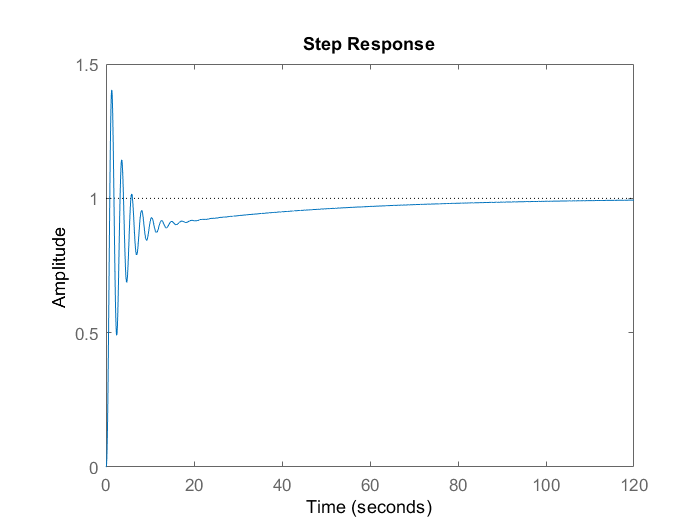
\includegraphics[width=\linewidth]{Step_PID_ZN}
		\caption{Step Response of the PID Controller Using Ziegler Nichols Tuning}
		\label{Step_PID_ZN}
	\end{figure}
		Now use MATLAB function stepinfo();, find the table of the step response characteristics as is shown in Table \ref{steptable_pid_zn} below. 
		\begin{table}[H]
			\centering
			\begin{tabular}{c c c c}
				$e_{ss}$ & $t_r$ & $t_s$ & $M_p$ \\
				0 & 0.513 & 76.420 & 40.386
			\end{tabular}
			\caption{Step Response Characteristic of the PID Controller Using Ziegler Nichols Tuning}
			\label{steptable_pid_zn}
		\end{table}
	
	\section{Conclusion}
		This lab investigated how a feedback control system can be used to modify a dynamic system. PID controllers are used in order to make different modifications. By controlling the parameters of the control plant, we can alter the rising time, settling time, steady-state error and the maximum overshoot of the step response of a close-loop system. In this way, we can modify the system according to different task requirements. Tuning methods are also investigated. By making use of the Bode Plot and the Root Locus plots, Ziegler Nichols Tuning method has proved to be able to find a suitable set of parameters for the PID controller. The built-in manual tuning tool in MATLAB also provides a powerful and visible approach for tuning the PID controllers.
	\section{Appendix: MATLAB Code for Modeling the PID Controller}
		\subsection{Analysis of the System with Transfer Function \textit{G(s)}}
			\begin{lstlisting}[frame=single, numbers=none]
G = tf([1], [1 6 11 6]);
figure(1)
hold on;
step(G);
stepinfo(G);
figure(2)
rlocus(G);
			\end{lstlisting}
		\subsection{Analysis of a Proportional Controller}
			\begin{lstlisting}[frame=single, numbers=none]
C_P = pid(40);
open_loop = series(C_P, G);
H1 = feedback(open_loop, 1);
hold on;
figure(1)
step(H1);
stepinfo(H1);
			\end{lstlisting}
		\subsection{PD Controller}
			\begin{lstlisting}[frame=single, numbers=none]
C_PD = pid(40, 0, 30);
open_loop_PD = series(C_PD, G);
H2 = feedback(open_loop_PD, 1);
hold on;
figure;
step(H2);
stepinfo(H2);
			\end{lstlisting}
		\subsection{PI Controller}
			\begin{lstlisting}[frame=single, numbers=none]
C_PD = pid(40, 10, 0);
open_loop_PD = series(C_PI, G);
H3 = feedback(open_loop_PI, 1);
hold on;
figure;
step(H3);
stepinfo(H3);
			\end{lstlisting}
		\subsection{PID Controller}
			\begin{lstlisting}[frame=single, numbers=none]
C_PD = pid(19, 12, 8);
open_loop_PD = series(C_PID, G);
H5 = feedback(open_loop_PID, 1);
hold on;
figure;
step(H5);
stepinfo(H5);
			\end{lstlisting}
		\subsection{Automatic PID Tuning with MATLAB}
			\begin{lstlisting}[frame=single, numbers=none]
% %%Question 2
% %CHOOSE ONE OF THE OPTIONS BELOW
opts = pidtuneOptions('DesignFocus', 'disturbance-rejection');
% opts = pidtuneOptions('DesignFocus', 'reference-tracking');
% opts = pidtuneOptions('DesignFocus', 'balanced');
% 
% %CHOOSE ONE OF THE OPTIONS BELOW
% type = 'P';
% type = 'I';
% type = 'PI';
% type = 'PD';
type = 'PID';
% 
C_auto = pidtune(G, type, opts);
open_loop_auto = series(C_auto, G);
H_auto = feedback(open_loop_auto, 1);
hold on;
figure(1);
step(H_auto);
stepinfo(H_auto);
			\end{lstlisting}
		\subsection{Complete Table of Step Response Characteristics of PID Controllers}
			\begin{table}[H]
				\centering
				\begin{tabular}{L | c c c c}
					Controller Type & $e_{ss}$ & $t_r$ & $t_s$ & $M_p$ \\
					\hline
					None & 83.33\% & 2.7428 & 5.0039 & 0\\
					P & 13.043\% & 0.4368 & 15.6105 & 67.6273\\
					PD & 13.043\% & 0.2494 & 1.4318 & 24.9544\\
					PI & 0 & 0.4593 & 23.6832 & 61.3913\\
					PID & 0 & 0.7352 & 1.7392 & 2.9293
				\end{tabular}
				\caption{Complete Table of Step Response Characteristics}
				\label{completeTable}
			\end{table}
\end{document}